\ofsubsection{Quebra de Limite}
%
\ofquote{"Esta é a cena em que você jura seu ódio eterno \\ por mim!"}{Seifer}\ofpar
%
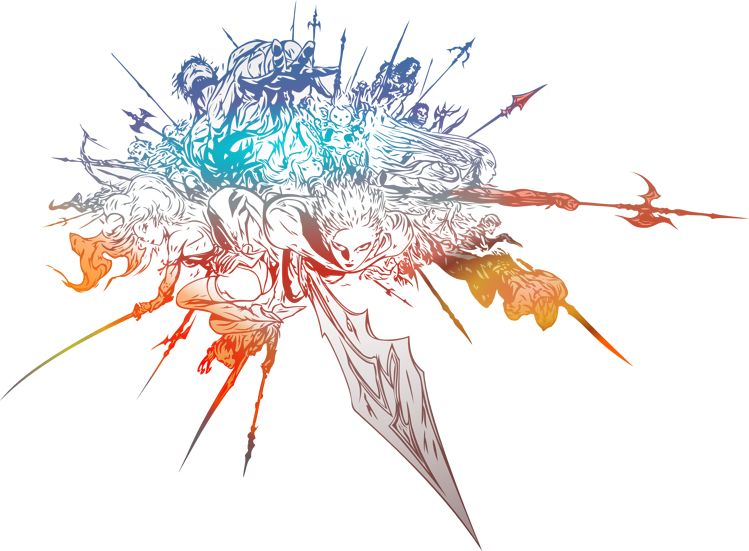
\includegraphics[width=\columnwidth]{./art/images/ff14.jpg}
%
\\\\\\
%
Em situações difíceis, herois podem ir além de seus limites e liberar habilidades poderosas, chamadas \accf{Quebra de Limite}.
Ao alcançarem o \accf{Nível~4}, os jogadores podem criar sua própria habilidade de Quebra de Limite.
Para usá-lo, o personagem tem que juntar 10 \accf{Pontos Limite~(PL)}, que serão consumidos ao ativar sua Quebra de Limite.
Cada jogador também escolhe um \accf{Modo Limite} para decidir sob quais circunstâncias seu personagem ganha PL, o que nunca excede 10 pontos.
Todos os Modos Limite disponíveis e suas condições d ganho de Pontos Limite estão na próxima página.
O MJ também pode permitir aos jogadores criarem suas próprias condições de Modo Limite.
A Quebra de Limite e o Modo Limite podem ser trocados a cada nível subsequente.
%
\ofpar\ofpar
%
\ofquote{"Quando um inimigo te irrita até o seu limite, você pode liberar um poder inimaginável."\\}{Cloud}
%
\ofpar
%
\ofboxwithtitle{Exemplo: Pontos Limite}{
	Vivi e seus amigos estão viajando em uma aeronave quando subitamente um mago hostil, chamado Valsa Negra, desce ao deque.
	O demônio causa KO a 5 passageiros imediatamente, usando uma poderosa magia de Raio. 
	Vivi selecionou o Modo Limite, Vingador, então ele ganha 10 pontos imediatamente ao assistir ao incidente.
	Ele jura se vingar e combater o monstro.
	Ele ativa sua Quebra de Limite, esvaziando sua Barra de Limite e recebendo poderosos benefícios de combate.
	A Quebra de Limite dá a Vivi e a seu grupo uma vantagem muito necessária na batalha que os permitem derrotar o poderoso inimigo em definitivo.
}
%
\newpage
%
Além de Modos Limite, todos os jogadores também ganham Pontos Limite nas seguintes situações: \ofrow
\ofbullet{3 PL após terminar uma batalha.}
\ofbullet{3 PL após acordar.}
\ofbullet{3 PL após usar um Talento.}
\ofbullet{10 PL após um aliado sofrer Ko e você for o último de pé.}
\ofbullet{10 PL após subir de Nível.}
\ofbullet{O MJ é encorajado a premiar PLs extras sempre que o personagem realiza um feito impressionante, heroico ou sempre que o grupo cumprir atividades ou missões importantes.}
%
\ofpar\\
%
\ofquote{"Vamos só atirar feito loucos e fazer um grande buraco, BOOM!"\\}{Selphie}
%
\ofpar
%
Quebra de Limite é usado da mesma maneira que Magia e Técnicas, mas sem custo de PM ou tempo de conjuração.
Você pode criar uma Quebra de Limite única ao escolher qualquer uma de suas magias ou técnicas como base.
Assim, adicione algumas melhorias e efeitos a fim de transformar a habilidade.
Cada efeito adicional aumenta o \accf{Grau~(GR)} de sua Quebra de Limite, que não pode exceder 5 pontos. 
Entretanto, não há benefício em ficar abaixo desse valor.
Por fim, escolha um novo nome para sua Quebra de Limite e visualize como ele é ao ser ativado.
Todas as possíveis melhorias que você possa usar para na criação, assim como o custo de Grau dela, estão listadas abaixo.
Você não pode escolher a mesma melhoria mais de uma vez, embora o MJ possa permitir outras opções além das listadas abaixo, atribuindo-lhes um Grau.
%
\ofpar\\
%
\ofboxwithtitle{Exemplo: Quebra de Limite}{
	Cloud, profissão Guerreiro, alcança o Nível 4, então ele pode criar sua própria Quebra de Limite.
	Ele escolhe sua habilidade Surrar como base, que permite ao usuário Atacar com menos precisão, garantindo um Acerto Crítico se acertar.
	Ele escolhe as seguintes melhorias até o Grau 5:
	\ofbullet{Mova-se até 3u antes ou depois de usar a habilidade.}
	\ofbullet{Ataques feitos durante a habilidade não podem ser evadidas.}
	\ofbullet{O dano causado ao alvo ignora DEF e RES.}
	\ofbullet{Alvos sofrem dano extra igual ao seu Nível atual.}
	Portanto, a nova habilidade o permite se reposicionar e então executar um Acerto Crítico, ignora a DEF e RES do alvo e causa 4 de dano extra. 
	Sendo uma Quebra de Limite, não há custo de PM ou tempo de conjuração.
	Cloud escolhe o nome Valente e o descreve da seguinte maneira:
	Você corre em direção ao alvo e antes de alcançá-lo, você salta no ar e executa um poderoso golpe de cima pra baixo. 
}
%
\clearpage
%
\oftable{p{0.22\columnwidth} p{0.06\columnwidth} p{0.65\columnwidth}}
{\accf{Modo Limite} & \accf{PL} & \accf{Condição}}
{
	Altruísta & 5 & Doe à caridade ou pessoa em necessidade. \ofrow
	Assaltante & 10 & Tenha uma rodada surpresa no combate. \ofrow
	Atleta & 5 & Malhe ou realize uma atividade física por pelo menos 1 hora. \ofrow
	Vingador & 4 & Um aliado que você vê sofre KO.\ofrow
	Traça & 5 & Leia ou estude por pelo menos 1 hora. \ofrow 
	Corajoso & 5 & Passe num teste com Desvantagem. \ofrow
	Covarde & 5 & Escape durante uma batalha.\ofrow
	Competitivo & 5 & Vença um jogo ou competição. \ofrow
	Criativo & 5 & Crie uma obra de arte.\ofrow
	Criminoso & 5 & Quebre a lei do local. \ofrow
	Culinária & 5 & Prepare e coma uma refeição gostosa.\ofrow
	Destemido & 5 & Ao fim da batalha seu PV está menos da metade.\ofrow
	Dominador & 5 & Ao fim da batalha seu PV está cheio. \ofrow
	Condutor & 5 & Conduza um veículo ou montaria por pelo menos 1 hora. \ofrow
	Elusivo & 2 & Evada-se de um ataque. \ofrow
	Explorador & 10 & Entre numa ruína, caverna, masmorra ou estrutura natural nova. \ofrow
	Ganancioso & 5 & Ganhe Gil ao completar tarefas.\ofrow
	%Pechinchador & 10 & Convença um mercador a dar um desconto ou pagar um preço maior por algo.\ofrow
	Útil & 5 & Crie ou repare um produto funcional. \ofrow
	Curandeiro & 4 & Remova KO de um aliado. \ofrow
	Solitário & 1 & seja escolhido por ultimo na ordem de turno de seu grupo. \ofrow
	Sortudo & 3 & Use um Dado de Fortuna. \ofrow
	Orador & 5 & Faça um discurso motivacional. \ofrow
	Pacifista & 5 & Evite o combate com sucesso. \ofrow
	Sombra & 5 & Esgueire-se por alguém sem ser notado.\ofrow
	Matador & 2 & Reduza um inimigo a 0 PV. \ofrow
	Sabotador & 2 & Inflija um Efeito de Estado em um ou mais inimigos. \ofrow
	Dorminhoco & 3 & Durma pelo menos 8 horas. \ofrow
	Espiritual & 4 & Realize um ritual ou prece religiosa. \ofrow
	Fornecedor & 1 & Use um Item.\ofrow
	Sociável & 2 & Tenha uma conversa com uma pessoa que não conheça.\ofrow
	Azarado & 4 & Falhe num teste com Vantagem. \ofrow
	Urbano & 10 & Entre numa vila, cidade pequena ou grande nova. \ofrow
	Vitimante & 5 & Sofra KO.\ofrow
	Andarilho & 5 & Ande a pé por pelo menos 1 hora. \ofrow
	Aquecimento & 1 & Use a habilidade na qual sua Quebra de Limite é baseada.
}
%
\newpage
%
\oftable{p{0.85\columnwidth} r}
{\accf{Efeito Adicional} & \accf{GR}}
{
	A habilidade ganha um tipo elemental que causa dano extra igual a metade de seu nível atual ao alvo. & +1 \ofrow
	Mude o tipo de dano causado entre Físico e Mágico. & +1 \ofrow
	Alvos sofrem dano extra igual ao seu nível atual. & +1 \ofrow
	Alvos recuperam PV igual ao seu nível atual. & +1 \ofrow
	A distância é aumentada em 3u. & +1 \ofrow
	Se os alvos tem de fazer um teste, o Quebra de Limite aumenta em 2. & +1 \ofrow
	Alvos se tornam Imunes a Efeitos de Estado à sua escolha por 3 rodadas. & +1 \ofrow
	Alvos recuperam PM igual ao seu nível atual. & +1 \ofrow
	Mova-se até 3u antes ou depois de usar uma habilidade. & +1 \ofrow
	Somente inimigos na área são afetados.  & +1 \ofrow
	Dano causado ignora a DEF e RES do alvo. & +1 \ofgap
	Dano causado ignora as Resistências do alvo. & +1 \ofgap
	A área alvo aumenta em 2u. & +2 \ofrow
	Recupere PM igual a duas vezes seu nível atual. & +2 \ofrow
	Empurre os alvos até 3u. & +2 \ofrow
	Tome a ação Defender após usar a habilidade.  & +2 \ofrow
	Efeitos com duração se estendem por mais 2 rodadas. & +2 \ofrow
	Alvos sofrem o Efeito de Estado escolhido por você, exceto KO, por 1 rodada. & +2 \ofrow
	Após usar a habilidade, faça um Ataque contra um alvo dentro do alcance. & +2 \ofrow
	Use a habilidade como reação sob condições específicas. Ex.: receba dano, a rodada termina, um inimigo entra ao seu alcance. & +2 \ofrow
	Use um item de seu inventário em adição. & +2 \ofrow
	O PM dos alvos é reduzido igual ao seu nível atual. & +2 \ofrow
	Ataques realizados por habilidades não podem ser evadidos. & +2 \ofrow
	Um aliado dentro de 3u pode usar uma habilidade conhecida no mesmo alvo sem custo adicional ou tempo de conjuração.  & +2 \ofrow
	Alvos sofrem dano extra igual a sua FOR ou MAG combinadas. & +2 \ofrow
	Alvos se tornam Imunes a Efeitos de Estado negativos por 3 rodadas. & +3 \ofrow
	Aja novamente após usar essa habilidade. & +3 \ofrow
	Crie um Campo à sua escolha que alcance até 3u ao redor do alvo e dure 3 rodadas. & +3 \ofrow
	Após usar a habilidade, ganhe AuFOR, AuMAG, AuDEF e AuRES por 3 rodadas. & +3 \ofrow
	Alvos ganham Resistência contra todos os tipos elementais por 3 rodadas. & +3
}
%
\clearpage